% Options for packages loaded elsewhere
\PassOptionsToPackage{unicode}{hyperref}
\PassOptionsToPackage{hyphens}{url}
%
\documentclass[
]{article}
\usepackage{amsmath,amssymb}
\usepackage{lmodern}
\usepackage{iftex}
\ifPDFTeX
  \usepackage[T1]{fontenc}
  \usepackage[utf8]{inputenc}
  \usepackage{textcomp} % provide euro and other symbols
\else % if luatex or xetex
  \usepackage{unicode-math}
  \defaultfontfeatures{Scale=MatchLowercase}
  \defaultfontfeatures[\rmfamily]{Ligatures=TeX,Scale=1}
\fi
% Use upquote if available, for straight quotes in verbatim environments
\IfFileExists{upquote.sty}{\usepackage{upquote}}{}
\IfFileExists{microtype.sty}{% use microtype if available
  \usepackage[]{microtype}
  \UseMicrotypeSet[protrusion]{basicmath} % disable protrusion for tt fonts
}{}
\makeatletter
\@ifundefined{KOMAClassName}{% if non-KOMA class
  \IfFileExists{parskip.sty}{%
    \usepackage{parskip}
  }{% else
    \setlength{\parindent}{0pt}
    \setlength{\parskip}{6pt plus 2pt minus 1pt}}
}{% if KOMA class
  \KOMAoptions{parskip=half}}
\makeatother
\usepackage{xcolor}
\usepackage[margin=1in]{geometry}
\usepackage{color}
\usepackage{fancyvrb}
\newcommand{\VerbBar}{|}
\newcommand{\VERB}{\Verb[commandchars=\\\{\}]}
\DefineVerbatimEnvironment{Highlighting}{Verbatim}{commandchars=\\\{\}}
% Add ',fontsize=\small' for more characters per line
\usepackage{framed}
\definecolor{shadecolor}{RGB}{248,248,248}
\newenvironment{Shaded}{\begin{snugshade}}{\end{snugshade}}
\newcommand{\AlertTok}[1]{\textcolor[rgb]{0.94,0.16,0.16}{#1}}
\newcommand{\AnnotationTok}[1]{\textcolor[rgb]{0.56,0.35,0.01}{\textbf{\textit{#1}}}}
\newcommand{\AttributeTok}[1]{\textcolor[rgb]{0.77,0.63,0.00}{#1}}
\newcommand{\BaseNTok}[1]{\textcolor[rgb]{0.00,0.00,0.81}{#1}}
\newcommand{\BuiltInTok}[1]{#1}
\newcommand{\CharTok}[1]{\textcolor[rgb]{0.31,0.60,0.02}{#1}}
\newcommand{\CommentTok}[1]{\textcolor[rgb]{0.56,0.35,0.01}{\textit{#1}}}
\newcommand{\CommentVarTok}[1]{\textcolor[rgb]{0.56,0.35,0.01}{\textbf{\textit{#1}}}}
\newcommand{\ConstantTok}[1]{\textcolor[rgb]{0.00,0.00,0.00}{#1}}
\newcommand{\ControlFlowTok}[1]{\textcolor[rgb]{0.13,0.29,0.53}{\textbf{#1}}}
\newcommand{\DataTypeTok}[1]{\textcolor[rgb]{0.13,0.29,0.53}{#1}}
\newcommand{\DecValTok}[1]{\textcolor[rgb]{0.00,0.00,0.81}{#1}}
\newcommand{\DocumentationTok}[1]{\textcolor[rgb]{0.56,0.35,0.01}{\textbf{\textit{#1}}}}
\newcommand{\ErrorTok}[1]{\textcolor[rgb]{0.64,0.00,0.00}{\textbf{#1}}}
\newcommand{\ExtensionTok}[1]{#1}
\newcommand{\FloatTok}[1]{\textcolor[rgb]{0.00,0.00,0.81}{#1}}
\newcommand{\FunctionTok}[1]{\textcolor[rgb]{0.00,0.00,0.00}{#1}}
\newcommand{\ImportTok}[1]{#1}
\newcommand{\InformationTok}[1]{\textcolor[rgb]{0.56,0.35,0.01}{\textbf{\textit{#1}}}}
\newcommand{\KeywordTok}[1]{\textcolor[rgb]{0.13,0.29,0.53}{\textbf{#1}}}
\newcommand{\NormalTok}[1]{#1}
\newcommand{\OperatorTok}[1]{\textcolor[rgb]{0.81,0.36,0.00}{\textbf{#1}}}
\newcommand{\OtherTok}[1]{\textcolor[rgb]{0.56,0.35,0.01}{#1}}
\newcommand{\PreprocessorTok}[1]{\textcolor[rgb]{0.56,0.35,0.01}{\textit{#1}}}
\newcommand{\RegionMarkerTok}[1]{#1}
\newcommand{\SpecialCharTok}[1]{\textcolor[rgb]{0.00,0.00,0.00}{#1}}
\newcommand{\SpecialStringTok}[1]{\textcolor[rgb]{0.31,0.60,0.02}{#1}}
\newcommand{\StringTok}[1]{\textcolor[rgb]{0.31,0.60,0.02}{#1}}
\newcommand{\VariableTok}[1]{\textcolor[rgb]{0.00,0.00,0.00}{#1}}
\newcommand{\VerbatimStringTok}[1]{\textcolor[rgb]{0.31,0.60,0.02}{#1}}
\newcommand{\WarningTok}[1]{\textcolor[rgb]{0.56,0.35,0.01}{\textbf{\textit{#1}}}}
\usepackage{graphicx}
\makeatletter
\def\maxwidth{\ifdim\Gin@nat@width>\linewidth\linewidth\else\Gin@nat@width\fi}
\def\maxheight{\ifdim\Gin@nat@height>\textheight\textheight\else\Gin@nat@height\fi}
\makeatother
% Scale images if necessary, so that they will not overflow the page
% margins by default, and it is still possible to overwrite the defaults
% using explicit options in \includegraphics[width, height, ...]{}
\setkeys{Gin}{width=\maxwidth,height=\maxheight,keepaspectratio}
% Set default figure placement to htbp
\makeatletter
\def\fps@figure{htbp}
\makeatother
\setlength{\emergencystretch}{3em} % prevent overfull lines
\providecommand{\tightlist}{%
  \setlength{\itemsep}{0pt}\setlength{\parskip}{0pt}}
\setcounter{secnumdepth}{5}
\ifLuaTeX
  \usepackage{selnolig}  % disable illegal ligatures
\fi
\IfFileExists{bookmark.sty}{\usepackage{bookmark}}{\usepackage{hyperref}}
\IfFileExists{xurl.sty}{\usepackage{xurl}}{} % add URL line breaks if available
\urlstyle{same} % disable monospaced font for URLs
\hypersetup{
  pdftitle={HUDM6122 Homework\_01},
  pdfauthor={Chenguang Pan},
  hidelinks,
  pdfcreator={LaTeX via pandoc}}

\title{HUDM6122 Homework\_01}
\author{Chenguang Pan}
\date{Jan 28, 2023}

\begin{document}
\maketitle

\hypertarget{exercise-1.1}{%
\subsection{Exercise 1.1}\label{exercise-1.1}}

First, I made a xlsx. version of \texttt{Table\ 1.1} to let R read it
directly using the package `readxl``. This table is in 10x7 size. The
first column is just the index of each observation, so I drop it here.
Finally this dataset is in 9x7 size.

One should notice that the \texttt{sex}, \texttt{depression}, and
\texttt{health} are categorical variables. The Pearson Correlation
Coefficient is used for continuous rather than categorical variables.
Therefore, when calculate the correlation matrix we should drop the
categorical ones.

Note, there are some parameters need to be set. Since the original
dataset contains missing value, I construct the correlation matrix based
on all complete observations.

\begin{Shaded}
\begin{Highlighting}[]
\SpecialCharTok{\textgreater{}} \FunctionTok{library}\NormalTok{(readxl)}
\SpecialCharTok{\textgreater{}}\NormalTok{ table\_11 }\OtherTok{\textless{}{-}} \FunctionTok{read\_excel}\NormalTok{(}\StringTok{"table\_1.1.xlsx"}\NormalTok{)}
\SpecialCharTok{\textgreater{}}\NormalTok{ my\_data }\OtherTok{\textless{}{-}}\NormalTok{ table\_11[,}\FunctionTok{c}\NormalTok{(}\DecValTok{2}\SpecialCharTok{:}\DecValTok{7}\NormalTok{)]}
\SpecialCharTok{\textgreater{}} \CommentTok{\# drop the discrete vars and use only the complete observations}
\ErrorTok{\textgreater{}}\NormalTok{ my\_data\_cor }\OtherTok{\textless{}{-}} \FunctionTok{round}\NormalTok{(}\FunctionTok{cor}\NormalTok{(my\_data[,}\FunctionTok{c}\NormalTok{(}\DecValTok{2}\NormalTok{,}\DecValTok{3}\NormalTok{,}\DecValTok{6}\NormalTok{)], }\AttributeTok{use =} \StringTok{"complete"}\NormalTok{),}\DecValTok{2}\NormalTok{)}
\SpecialCharTok{\textgreater{}} \CommentTok{\# the output is rounded in two decimals.}
\ErrorTok{\textgreater{}}\NormalTok{ my\_data\_cor}
\NormalTok{         age    IQ weight}
\NormalTok{age     }\FloatTok{1.00} \SpecialCharTok{{-}}\FloatTok{0.15}  \SpecialCharTok{{-}}\FloatTok{0.12}
\NormalTok{IQ     }\SpecialCharTok{{-}}\FloatTok{0.15}  \FloatTok{1.00}   \FloatTok{0.75}
\NormalTok{weight }\SpecialCharTok{{-}}\FloatTok{0.12}  \FloatTok{0.75}   \FloatTok{1.00}
\end{Highlighting}
\end{Shaded}

\hypertarget{exercise-1.2}{%
\subsection{Exercise 1.2}\label{exercise-1.2}}

Fill the \texttt{NA} with the column's mean, and recalculate the
correlation matrix.

\begin{Shaded}
\begin{Highlighting}[]
\SpecialCharTok{\textgreater{}} \CommentTok{\# to impute the NA with mean using a for{-}loop}
\ErrorTok{\textgreater{}} \ControlFlowTok{for}\NormalTok{ (cols }\ControlFlowTok{in} \FunctionTok{c}\NormalTok{(}\DecValTok{2}\NormalTok{,}\DecValTok{3}\NormalTok{,}\DecValTok{6}\NormalTok{)) \{}
\SpecialCharTok{+}\NormalTok{   my\_data[,cols][}\FunctionTok{is.na}\NormalTok{(my\_data[,cols])] }\OtherTok{\textless{}{-}} \FunctionTok{mean}\NormalTok{(my\_data[,cols], }\AttributeTok{na.rm=}\NormalTok{T)}
\SpecialCharTok{+}\NormalTok{ \}}
\SpecialCharTok{\textgreater{}} \CommentTok{\# create the correlation matrix}
\ErrorTok{\textgreater{}}\NormalTok{ my\_data\_cor\_2 }\OtherTok{\textless{}{-}} \FunctionTok{round}\NormalTok{(}\FunctionTok{cor}\NormalTok{(my\_data[,}\FunctionTok{c}\NormalTok{(}\DecValTok{2}\NormalTok{,}\DecValTok{3}\NormalTok{,}\DecValTok{6}\NormalTok{)]),}\DecValTok{2}\NormalTok{)}
\SpecialCharTok{\textgreater{}}\NormalTok{ my\_data\_cor\_2 }
\NormalTok{         age    IQ weight}
\NormalTok{age     }\FloatTok{1.00} \SpecialCharTok{{-}}\FloatTok{0.14}  \SpecialCharTok{{-}}\FloatTok{0.10}
\NormalTok{IQ     }\SpecialCharTok{{-}}\FloatTok{0.14}  \FloatTok{1.00}   \FloatTok{0.52}
\NormalTok{weight }\SpecialCharTok{{-}}\FloatTok{0.10}  \FloatTok{0.52}   \FloatTok{1.00}
\end{Highlighting}
\end{Shaded}

\hypertarget{exercise-1.3}{%
\subsection{Exercise 1.3}\label{exercise-1.3}}

The authors may not clearly say where can readers find the original
dataset. After seeing the code underlying in this book's R package
\texttt{MVA}, and run this argument \texttt{demo("Ch-MVA")}, one can
find the \texttt{table\ 1.3}'s dataset information at the paragraph
named \texttt{code\ chunk\ number\ 5}. It is in another package called
\texttt{HSAUR2}.

\begin{Shaded}
\begin{Highlighting}[]
\SpecialCharTok{\textgreater{}} \CommentTok{\# load the Table 1.3\textquotesingle{}s original dataset }
\ErrorTok{\textgreater{}} \FunctionTok{library}\NormalTok{(HSAUR2)}
\SpecialCharTok{\textgreater{}} \FunctionTok{dim}\NormalTok{(pottery)}
\NormalTok{[}\DecValTok{1}\NormalTok{] }\DecValTok{45} \DecValTok{10}
\SpecialCharTok{\textgreater{}} \FunctionTok{names}\NormalTok{(pottery) }\CommentTok{\# the dataset is the same}
\NormalTok{ [}\DecValTok{1}\NormalTok{] }\StringTok{"Al2O3"} \StringTok{"Fe2O3"} \StringTok{"MgO"}   \StringTok{"CaO"}   \StringTok{"Na2O"}  \StringTok{"K2O"}   \StringTok{"TiO2"}  \StringTok{"MnO"}   \StringTok{"BaO"}  
\NormalTok{[}\DecValTok{10}\NormalTok{] }\StringTok{"kiln"} 
\SpecialCharTok{\textgreater{}} \CommentTok{\# par(mfrow = c(4,3))}
\ErrorTok{\textgreater{}} \ControlFlowTok{for}\NormalTok{ (i }\ControlFlowTok{in} \FunctionTok{c}\NormalTok{(}\DecValTok{1}\SpecialCharTok{:}\FunctionTok{length}\NormalTok{(}\FunctionTok{ncol}\NormalTok{(pottery))))\{}
\SpecialCharTok{+}\NormalTok{   col\_name }\OtherTok{\textless{}{-}} \FunctionTok{colnames}\NormalTok{(pottery)[i]}
\SpecialCharTok{+}   \FunctionTok{qqnorm}\NormalTok{(pottery[,i],}
\SpecialCharTok{+}          \AttributeTok{xlab =} \StringTok{"Normal Scores"}\NormalTok{,}
\SpecialCharTok{+}          \AttributeTok{main =}\NormalTok{ col\_name)}
\SpecialCharTok{+}   \FunctionTok{qqline}\NormalTok{(pottery[, i])}
\SpecialCharTok{+}\NormalTok{   \}}
\end{Highlighting}
\end{Shaded}

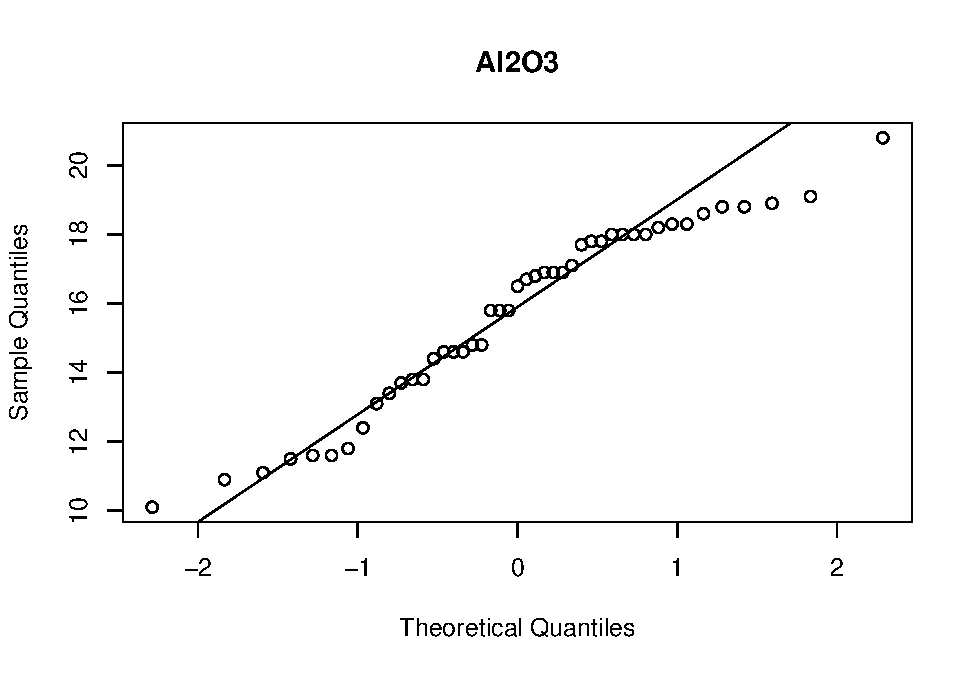
\includegraphics{hudm6122_hw_01_ChenguangPan_files/figure-latex/unnamed-chunk-3-1.pdf}

\end{document}
